\section{Enemy}

This class implements the Behavior for the Enemy of the game. its AI is defined as 
state machine, represented in figure \ref{fig:enemy_AI}, and thus the update method is divided in the various states it can be. 

\begin{figure}[h]
    \centering
    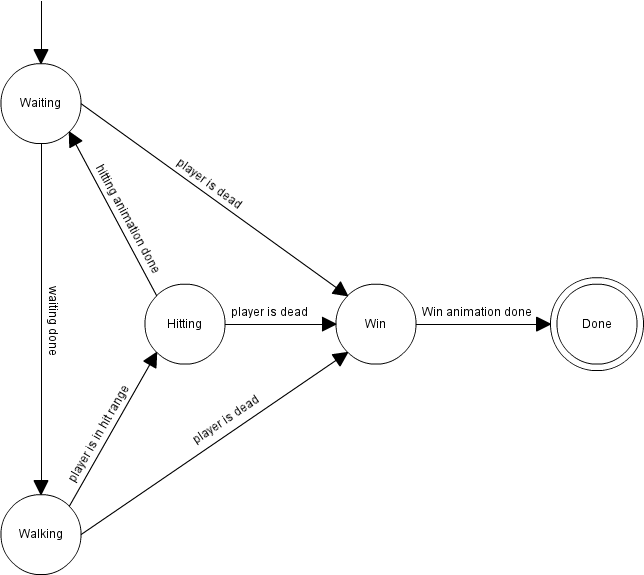
\includegraphics[width=0.8\textwidth]{enemy_AI}
    \caption{Flow chart of the Enemy's AI}
    \label{fig:enemy_AI}
\end{figure}

\begin{lstlisting}
#ifndef ENEMY_HPP
#define ENEMY_HPP
#include "hummingbird/hum.hpp"
#include "MOGL/MOGL.hpp"
#include "Resources.hpp"
#include "Player.hpp"
#include "math.hpp"

class Enemy : public hum::Behavior
{
private:
    enum State { WALKING, HITTING, WAITING, WIN, DONE };

    static float s_vel;
    static float s_min_player_dist;

    hum::Clock p_clock;
    State p_status;
    Player* p_player;
    hum::Kinematic* p_kinematic;
    float p_prev_rotation;
    mogl::AnimatedSprite* p_sprite;
    mogl::AnimatedSprite* p_blood;
    mogl::MultimediaOGL* p_mogl;
    mogl::SoundId p_sound;

public:
    // Enemy's AI states
    enum State { WALKING, HITTING, WAITING, WIN, DONE };

    Enemy(Player* player):
    p_player(player),
    p_sound(0)
    {
        if (s_vel == -1)
        {
            std::stringstream ss;
            readFileContents("res/config/Enemy.cfg", ss);
            ss >> s_vel;
            ss >> s_min_player_dist;
        }
    }
\end{lstlisting}

As in the Player class, we include the required files, define private variables to 
store useful information and use the constructor for reading the class configuration. Some 
of the private information is similar to the player's one.

Enemy receives a pointer to the player in its constructor, we store it. We'll use it 
to check if the player is in hitting range and if so hit it.

Unlike Player, Enemy has two AnimatedSprites. The first is the one that plays the various 
enemy animations: walking, hitting, winning; the second plays the blood animation, only 
show when the player is hit. Finally, the we store a SoundId to handle the playback of 
the various sounds the Enemy can produce: hit and roar.

\begin{lstlisting}
    void init() override
    {
        p_kinematic = actor().addBehavior<hum::Kinematic>();
        p_prev_rotation = 0;

        p_mogl = actor().game().getPlugin<mogl::MultimediaOGL>();
        p_sprite = actor().addBehavior<mogl::AnimatedSprite>(p_mogl->spriteAnimations().get("enemy_walking"));
        p_sprite->pause();
        p_sprite->setOrigin(hum::Vector3f(24./48., 18./48., 0));
        actor().transform().rotation.z = -90;

        p_blood = actor().addBehavior<mogl::AnimatedSprite>(p_mogl->spriteAnimations().get("enemy_attack1_blood"));
        p_blood->setLooping(false);
        p_blood->stop();
        p_blood->disable();
        p_blood->setOrigin(hum::Vector3f(24./48., -10./24., 0));

        p_status = WAITING;
    }
\end{lstlisting}

Like in Player, we use the initialitazion method for configuring the actor. We add 
the Kinematic Behavior and the AnimatedSprites, setting each of them accordingly. Finally, 
we set the initial AI state.

Enemy also needs to handle its destruction, as it uses sound resources. We release them, 
by stoping the sound we indicate it is done and MOGL will take care of freeing it.

\begin{lstlisting}
    void onDestroy() override
    {
        if (p_mogl->sounds().get(p_sound) != nullptr)
        {
            p_mogl->sounds().get(p_sound)->stop();
        }
    }
\end{lstlisting}

Now it is when the fun comes: the update. The first thing we do is to define the \textit{base} 
state changes: if the Enemy is \textbf{done}, do nothing; and if the player dies, 
change to \textbf{win} state.

In the \textbf{win} state, the Enemy does nothing, just waits one second still. Therefore, we 
stop all animations and reset the clock to mesure the second.

\begin{lstlisting}
    void fixedUpdate() override
    {
        if (p_status == DONE)
        {
            return;
        }

        if (p_player->isDead() and p_status != DONE and p_status != WIN)
        {
            p_status = WIN;
            p_sprite->stop();
            p_blood->disable();
            p_clock.reset();
        }
\end{lstlisting}

Next, we calculate the rotation speed of the Enemy. This step is the same as the player, 
with the difference that the position to look at is not the mouse but the player. We 
also calculate the distance between the enemy and the player and set the speed of the 
enemy to 0.

\begin{lstlisting}

        // Look at the player
        float x = p_player->actor().transform().position.x - actor().transform().position.x;
        float y = p_player->actor().transform().position.y - actor().transform().position.y;
        float angleInRadians = std::atan2(y, x);
        float angleInDegrees = (angleInRadians / M_PI) * 180.0;
        float delta = angleInDegrees - p_prev_rotation;
        if (delta > 180)
        {
            delta -= 360;
        }
        else if (delta < -180)
        {
            delta += 360;
        }
        p_kinematic->velocity().rotation.z = delta / actor().game().fixedUpdateTime().asSeconds();
        p_prev_rotation = angleInDegrees;

        p_kinematic->velocity().position.x = 0;
        p_kinematic->velocity().position.y = 0;

        // distance between the enemy and the player
        float mod = sqrt(square(x) + square(y));
\end{lstlisting}

If the enemy is in \textbf{win} state and the one second still time has passed, the 
enemy changes to \textbf{done} state and starts the win animation. We set the animation 
not to loop so that it stops when done.

\begin{lstlisting}
        if (p_status == WIN)
        {
            if (p_clock.getTime().asSeconds() > 1)
            {
                p_sprite->setSpriteAnimation(p_mogl->spriteAnimations().get("enemy_win"));
                p_sprite->setLooping(false);
                p_sprite->play();
                p_status = DONE;
            }
        }
\end{lstlisting}

On the other hand, if the enemy is \textbf{walking} and the player is not in hitting range 
the enemy moves towards the player. We set the speed, play the walking animation if 
not playing already and, with a probability of 0.01, play the \textit{roar} sound if 
no sound is playing. We store the SoundId of the roar sound so that we know if the 
enemy is still roaring or not.

\begin{lstlisting}
        else if (p_status == WALKING and s_min_player_dist < mod)
        {
            x /= mod;
            y /= mod;
            p_kinematic->velocity().position.x = x * s_vel;
            p_kinematic->velocity().position.y = y * s_vel;
            if (p_sprite->status() != mogl::AnimatedSprite::Status::PLAYING)
            {
                p_sprite->play();
            }

            if (p_mogl->sounds().get(p_sound) == nullptr and (rand()%100) > 99)
            {
                auto info = p_mogl->sounds().play("roar", 1000);
                info.second->setAttenuation(0.1);
                p_sound = info.first;
            }
        }
        else
        {
            if (p_status != WAITING)
            {
                if (p_status != HITTING) // state == WALKING and player is in hitting distance
                {
\end{lstlisting}

If the enemy is \textbf{walking} and the player is in hitting distance, the enemy changes 
to \textit{hitting} state. Changes the animation of the sprite and sets it not to loop, 
this way we can check when the animation is done and change to the next state. Finally, 
we play the sound of the enemy's attack and set its position and attenuation. In this case, 
we don't need to store the SoundId because we know that the hit sound will finish before the 
enemy is able to hit again.

\begin{lstlisting}
                    p_sprite->setSpriteAnimation(p_mogl->spriteAnimations().get("enemy_attack1"));
                    p_sprite->play();
                    p_sprite->setLooping(false);
                    p_status = HITTING;
                    sf::Sound* sound = p_mogl->sounds().play("enemy_attack", 50).second;
                    sound->setPosition(actor().transform().position.x, actor().transform().position.y, 0);
                    sound->setAttenuation(0.01);
                }
                else
                {
\end{lstlisting}

If the state is \textbf{hitting} and the hitting animation has finished, the status 
changes to \textbf{waiting}. We set the animation back to walking and disable the blood 
AnimatedSprite, in case it was displayed. The clock is also resetted so that we can mesure 
the waiting time.

\begin{lstlisting}
                    if (p_sprite->status() == mogl::AnimatedSprite::Status::STOPPED)
                    {
                        p_sprite->setSpriteAnimation(p_mogl->spriteAnimations().get("enemy_walking"));
                        p_sprite->setLooping(true);
                        p_status = WAITING;

                        p_blood->stop();
                        p_blood->disable();

                        p_clock.reset();
                    }
\end{lstlisting}

Else, if the hitting animation hasn't finished but it just passed the frame where the 
hit happens, check if the player is still in range and if so, hit it and display blood.

\begin{lstlisting}
                    else if (p_sprite->frameIndex() > 1 and not p_blood->isEnabled())
                    {
                        if (mod < s_min_player_dist)
                        {
                            p_blood->enable();
                            p_blood->play();
                            p_player->hit();
                        }
                    }
                }
            }
            else
            {
\end{lstlisting}

Finally, if the enemy is in \textbf{waiting} state, check if the waiting time has 
passed and if so, set the state to \textbf{walking}.

\begin{lstlisting}
                hum::Time t = p_clock.getTime();
                if (t.asSeconds() > 1)
                {
                    p_status = WALKING;
                }
            }
        }
\end{lstlisting}

As a last detail, if the \textit{roar} sound is being played, update its position.
\begin{lstlisting}
        sf::Sound* sound = p_mogl->sounds().get(p_sound);
        if (sound != nullptr)
        {
            sound->setPosition(actor().transform().position.x, actor().transform().position.y, 0);
        }
    }

    static const char* behaviorName()
    {
        return "Enemy";
    }
};
float Enemy::s_vel = -1;
float Enemy::s_min_player_dist = -1;
#endif
\end{lstlisting}
